\begin{figure}[h]
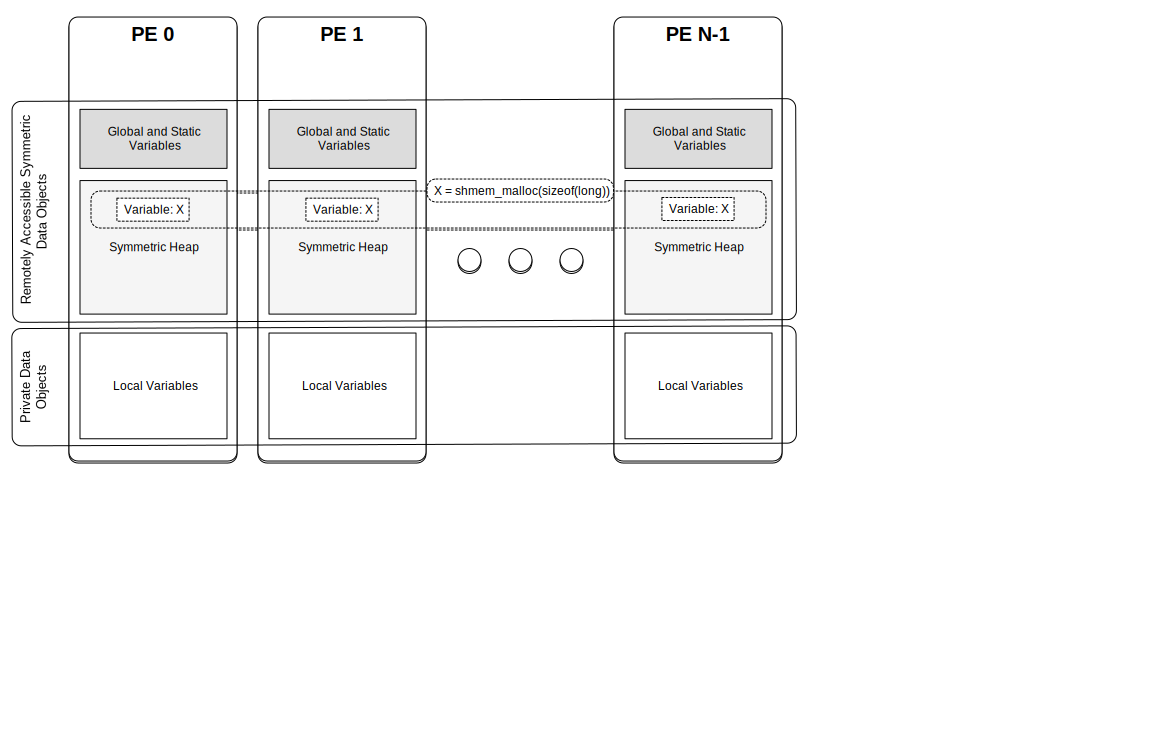
\includegraphics[width=0.95\textwidth]{figures/mem_model}
\caption{\openshmem Memory Model}
\label{fig:mem_model}
\end{figure}

\subsection{Object Storage Model}

An \openshmem program consists of data objects that are private to each \ac{PE}
and data  objects that are remotely accessible by all \acp{PE}. Private data
objects are stored in the local memory of each \ac{PE} and can only be accessed
by the \ac{PE} itself; these data objects cannot be accessed by other \acp{PE}
via \openshmem routines. Private data objects follow the memory model of
\Cstd. Remotely accessible objects, however, can be accessed by
remote \acp{PE} using \openshmem routines.  Remotely accessible data objects are
called \emph{Symmetric Data Objects}.  Each symmetric data object has a
corresponding object with the same name, type, and size on all \acp{PE} where that object is
accessible via the \openshmem \ac{API}\footnote{For efficiency reasons,
the same offset (from an arbitrary memory address) for symmetric data
objects might be used on all \acp{PE}. Further discussion about symmetric heap
layout and implementation efficiency can be found in Section~\ref{subsec:shfree}}.
(For the definition of what is accessible, see the
descriptions for \FUNC{shmem\_pe\_accessible} and \FUNC{shmem\_addr\_accessible}
in Sections~\ref{subsec:shmem_pe_accessible} and
\ref{subsec:shmem_addr_accessible}.) In \openshmem the following kinds of
data objects are symmetric:
%
\begin{itemize}
\item Global and static \Cstd and \Cpp variables \emph{not} defined in
  a dynamic shared object (DSO).
\item \Cstd and \Cpp data allocated by \openshmem memory management routines
  (Section~\ref{sec:memory_management})
\end{itemize}

\openshmem dynamic memory allocation routines (e.g.,
\FUNC{shmem\_malloc}) allow collective allocation of \emph{Symmetric Data
Objects} on a special memory region called the \emph{Symmetric Heap}. The
Symmetric Heap is created during the execution of a program at a memory location
determined by the implementation. The Symmetric Heap may reside in different
memory regions on different \acp{PE}.
Figure~\ref{fig:mem_model} shows an example \openshmem
memory layout, illustrating the location of remotely accessible symmetric
objects and private data objects.  As shown, symmetric data objects can be
located either in the symmetric heap or in the global/static memory section of
each \ac{PE}.

\subsubsection{Pointers to Symmetric Objects}\label{subsec:pointers_to_symmetric_objects}

Symmetric data objects are referenced in \openshmem operations through the
local pointer to the desired remotely accessible object.  The address contained
in this pointer is referred to as a {\em symmetric address}.  Every symmetric
address is also a {\em local address} that is valid for direct memory access;
however, not all local addresses are symmetric.  Manipulation of symmetric
addresses passed to \openshmem routines---including pointer arithmetic,
array indexing, and access of structure or union members---are permitted as long as
the resulting local pointer remains within the same symmetric allocation or
object.  Symmetric addresses are only valid at the \ac{PE} where they were
generated; using a symmetric address generated by a different \ac{PE} for
direct memory access or as an argument to an \openshmem routine results
in undefined behavior.

Symmetric addresses provided to typed and type-generic \openshmem interfaces
must be naturally aligned based on their type and any requirements of the
underlying architecture.  Symmetric addresses provided to fixed-size \openshmem
interfaces (e.g., \FUNC{shmem\_put32}) must also be aligned to the given
size.  Symmetric objects provided to fixed-size \openshmem interfaces
must have storage size equal to the bit-width of the given
operation\footnote{The bit-width of a byte is implementation-defined in \Cstd.  The
\CONST{CHAR\_BIT} constant in \HEADER{limits.h} can be used to portably
calculate the bit-width of a \Cstd object.}.  Because \CorCpp{} structures may
contain implementation-defined padding, the fixed-size interfaces should not be
used with \CorCpp{} structures.
The ``mem'' interfaces (e.g., \FUNC{shmem\_putmem}) have no alignment
requirements.

The \FUNC{shmem\_ptr} routine allows the programmer to query a {\em local
address} to a remotely accessible data object at a specified \ac{PE}.  The
resulting pointer is valid for direct memory access; however, providing this
address as an argument of an \openshmem routine that requires a symmetric
address results in undefined behavior.

\subsection{Synchronization, Ordering, and Consistency}

An \openshmem program can have one or more processes of execution
called \acp{PE}.  The execution of the entire \openshmem program
consists of the execution of all of its \acp{PE}.

The \openshmem memory model extends the defined behavior for the \Cstd
language (notably, that specified in \Cstd[11]/\Cstd[17] $\S$5.1.2.4
and $\S$7.17) for multi-\ac{PE} execution as follows:

\begin{enumerate}

\item \openshmem provides a set of \emph{synchronization operations}
  % (cf. \Cstd[17]~$\S$5.1.2.4-5)
  that ensure updates from one \ac{PE} are visible
  to another \ac{PE}:

  \begin{itemize}
  \item Atomic operations or \acp{AMO}
  \item Quiet and fence operations
  \item Wait operations
  \item Lock operations
  \end{itemize}

%% \item Two \openshmem operations \emph{conflict} if one of them
%%   modifies a memory location (local or symmetric) and the other reads
%%   or modifies the same memory location.

%% \item An \openshmem operation and an expression evaluation
%%   \emph{conflict} if one of them modifies a memory location and the
%%   other reads or modifies the same memory location.

%% \item The execution of an \openshmem program contains a \emph{data
%%   race} if it contains to conflicting operations

\item No \ac{RMA} operations are synchronizing operations.

\item All \openshmem atomic operations are performed as with the
  memory ordering \VAR{memory\_order\_relaxed}.

%% \item The execution of a program contains a \emph{data race} if it
%%   contains two conflicting actions in different \acp{PE}, at least one
%%   of which is not atomic, and neither happens before the other. Any
%%   such data race results in undefined behavior.

\item The \FUNC{shmem\_fence} operation is performed as with the
  memory ordering \VAR{memory\_order\_acq\_rel}.

\item The \FUNC{shmem\_quiet} operation is performed as with the
  memory ordering \VAR{memory\_order\_seq\_cst}.

\item An evaluation $A$ on \ac{PE}~$X$ \emph{\ac{PE}-happens-before}
  an evaluation $B$ on \ac{PE}~$Y$ when $A$
  \emph{\ac{PE}-synchronizes-with} $B$, or
  \begin{itemize}
  \item $A$ happens-before some evaluation $C$ on \ac{PE}~$X$,
  \item $C$ happens-before $B$ on \ac{PE}~$Y$,
  \item $C$ is a \FUNC{shmem\_team\_\{barrier, sync\}} operation on
    team $T$, and
  \item \acp{PE}~$X$ and $Y$ are in $T$
  \end{itemize}

%% \item A release fence $R$ in \ac{PE}~$X$ synchronizes-with an acquire
%%   operation $A$ in \ac{PE}~$Y$ if:
%%   \begin{itemize}
%%   \item \ac{PE}~$X$ performs an atomic update $U$ of the symmetric
%%     object $M$ on \ac{PE}~$Y$ via context $C$, and
%%   \item The release fence $R$ is either a:
%%     \begin{itemize}
%%     \item \FUNC{shmem\_fence} operation on context $C$ when $U$ is a
%%       blocking \ac{AMO}, or
%%     \item \FUNC{shmem\_quiet} operation on context $C$ when $U$ is a
%%       blocking or nonblocking \ac{AMO}
%%     \end{itemize}
%%     and
%%   \item $R$ is sequenced-before $U$, and
%%   \item The acquire operation $A$ on \ac{PE}~$Y$ is one of:
%%     \begin{itemize}
%%     \item \FUNC{shmem\_\{test,wait\_until\}} operation on $M$
%%     \item \FUNC{shmem\_\{test,wait\_until\}\_\{all,any,some\}[\_vector]}
%%       operation in which $M$ is an element on the array of variables
%%       being tested or waited upon.
%%     \end{itemize}
%%   \end{itemize}

%% \item A release fence $F_{\textrm{release}}$ in \ac{PE}~$X$
%%   synchronizes-with an acquire fence $F_{\textrm{acquire}}$ in
%%   \ac{PE}~$Y$ if:
%%   \begin{itemize}
%%   \item \ac{PE}~$X$ performs an updating \ac{AMO}
%%     $A_{\textrm{update}}$ of the symmetric object $M$ on \ac{PE}~$Y$
%%     via context $C$, and
%%   \item The release fence $F_{\textrm{release}}$ is either a:
%%     \begin{itemize}
%%     \item \FUNC{shmem\_fence} operation on context $C$ when
%%       $A_{\textrm{update}}$ is a blocking \ac{AMO}, or
%%     \item \FUNC{shmem\_quiet} operation on context $C$ when
%%       $A_{\textrm{update}}$ is a blocking or nonblocking \ac{AMO}, 
%%     \end{itemize}
%%     and
%%   \item $F_{\textrm{release}}$ is sequenced-before
%%     $A_{\textrm{update}}$ in \ac{PE}~$X$, and
%%   \item \ac{PE}~$Y$ performs a fetching \ac{AMO} $A_{\textrm{fetch}}$
%%     of the symmetric object $M$ on itself via context $D$, and
%%   \item The acquire fence $F_{\textrm{acquire}}$ is either a:
%%     \begin{itemize}
%%     \item \FUNC{shmem\_fence} operation on context $D$ when
%%       $A_{\textrm{fetch}}$ is a blocking \ac{AMO}, or
%%     \item \FUNC{shmem\_quiet} operation on context $D$ when
%%       $A_{\textrm{fetch}}$ is a blocking or nonblocking \ac{AMO}
%%     \end{itemize}
%%     and
%%   \item $A_{\textrm{fetch}}$ is sequenced-before
%%     $F_{\textrm{acquire}}$ in \ac{PE}~$Y$.
%%   \end{itemize}

%%   %% TODO: shmem_{clear,set,test}_lock

%% \item A release operation in \ac{PE}~$X$ synchronizes-with an acquire
%%   operation in \ac{PE}~$Y$ under the following conditions:
%%   \begin{itemize}
%%   \item The release operation is one of:
%%     \begin{itemize}
%%     \item A release fence $F_{\mathrm{release}}$ that is
%%       sequenced-before an updating \ac{AMO} $A_{\mathrm{update}}$
%%       issued on context $C$ of a symmetric object $M$ on \ac{PE}~$Y$
%%       when $F_{\mathrm{release}}$ is a(n):
%%       \begin{itemize}
%%       \item \FUNC{shmem\_fence} operation on context $C$ when
%%         $A_{\textrm{update}}$ is a blocking \ac{AMO}, or
%%       \item \FUNC{shmem\_quiet} operation on context $C$ when
%%         $A_{\textrm{update}}$ is a blocking or nonblocking \ac{AMO},
%%         or
%%       %% \item \openshmem operation that internally performs an operation
%%       %%   equivalent to \FUNC{shmem\_quiet} on the default context, $C$
%%       %%   is the the default context (e.g., \tex), and $A_{\textrm{update}}$ is a
%%       %%   blocking or nonblocking \ac{AMO}
%%       \end{itemize}
%%     \item A \FUNC{shmem\_clear\_lock} operation on the symmetric lock
%%       object $L$
%%     \end{itemize}
%%   \item The acquire operation is one of:
%%     \begin{itemize}
%%     \item A fetching \ac{AMO} $A_{\mathrm{fetch}}$ on that is
%%       sequenced-before an acquire fence $F_{\mathrm{acquire}}$
%%     \item \FUNC{shmem\_\{test,wait\_until\}} operation on $M$
%%     \item \FUNC{shmem\_\{test,wait\_until\}\_\{all,any,some\}[\_vector]}
%%       operation in which $M$ is an element on the array of variables
%%       being tested or waited upon.
%%     \item A \FUNC{shmem\_set\_lock} operation on the symmetric lock
%%       object $L$ returns, or a \FUNC{shmem\_test\_lock} operation on
%%       $L$ returns 0.
%%     \end{itemize}
%%   \end{itemize}

\item A release operation issued by \ac{PE}~$X$
  \ac{PE}-synchronizes-with an acquire operation issued by \ac{PE}~$Y$
  through a symmetric object $M$ on \ac{PE}~$Y$ when:
  \begin{itemize}
  \item The release operation is a release fence
    $F_{\mathrm{release}}$ issued on context $C$ that is
    sequenced-before an \ac{AMO} $A_{\mathrm{update}}$
    % issued on context $D$
    that updates a symmetric object $M$ on \ac{PE}~$Y$,
    and
    %% \begin{itemize}
    %% \item when $F_{\mathrm{release}}$ is a \FUNC{shmem\_fence}
    %%   operation on context $C$ and $A_{\textrm{update}}$ is a
    %%   blocking \ac{AMO}, or
    %% \item when $F_{\mathrm{release}}$ is a \FUNC{shmem\_quiet}
    %%   operation on context $C$ and $A_{\textrm{update}}$ is a blocking
    %%   or nonblocking \ac{AMO}
    %% \end{itemize}
    %% and,
  \item The acquire operation is one of:
    \begin{itemize}
    \item A fetching \ac{AMO} $A_{\mathrm{fetch}}$ on $M$ that is
      sequenced-before an acquire fence $F_{\mathrm{acquire}}$
    \item \FUNC{shmem\_\{test,wait\_until\}} operation on $M$
    \item \FUNC{shmem\_\{test,wait\_until\}\_\{all,any,some\}[\_vector]}
      operation in which $M$ is an element on the array of variables
      being tested or waited upon.
    \end{itemize}
  \end{itemize}
  %% As a result, all put and updating \ac{AMO} operations issued by
  %% \ac{PE}~$X$ on context $C$ \ac{PE}-happen-before all get and fetching
  %% \ac{AMO} operations issued by \ac{PE}~$Y$ to the same
  As a result, when $F_{\mathrm{release}}$ is:
  \begin{itemize}
  \item \FUNC{shmem\_fence}, all blocking put and updating \ac{AMO}
    operations sequenced-before \FUNC{shmem\_fence} and issued on
    context $C$ to \ac{PE}~$Y$ will \ac{PE}-happen-before all load,
    get (blocking or nonblocking), and fetching \ac{AMO} operations
    from the same locations on \ac{PE}~$Y$ that are sequenced-after
    the acquire operation.
  \item \FUNC{shmem\_quiet}, all put and updating \ac{AMO} operations
    (blocking or nonblocking) sequenced-before \FUNC{shmem\_quiet} and
    issued on context $C$ to any \ac{PE} will \ac{PE}-happen-before
    all load, get (blocking or nonblocking), and fetching \ac{AMO}
    operations from the same locations that are sequenced-after the
    acquire operation.
  \end{itemize}

%% \item A release operation issued by \ac{PE}~$X$
%%   \ac{PE}-synchronizes-with an acquire operation issued by \ac{PE}~$Y$
%%   through a symmetric object $M$ on a third \ac{PE}~$Z$ in the
%%   following cases:
%%   \begin{itemize}
%%   \item The release operation is a \FUNC{shmem\_quiet} operation that
%%     is sequenced-before an \ac{AMO} $A_{\mathrm{update}}$ issued on
%%     context $C$ that updates a symmetric object $M$ on \ac{PE}~$Z$
%%     when $F_{\mathrm{release}}$ is a \FUNC{shmem\_quiet} operation on
%%     context $C$ and $A_{\textrm{update}}$ is a blocking or nonblocking
%%     \ac{AMO}, and
%%   \item The acquire operation is one of:
%%     \begin{itemize}
%%     \item An \ac{AMO} $A_{\mathrm{fetch}}$ issued on context $D$ that
%%       fetches the value of the symmetric object $M$ from \ac{PE}~$Z$
%%       that is sequenced-before an acquire fence $F_{\mathrm{acquire}}$
%%     \end{itemize}
%%   \end{itemize}

\item There is a single, total order of all operations on a symmetric
  lock object $L$ such that a lock-release operation (i.e.,
  \FUNC{shmem\_clear\_lock}) issued by \ac{PE}~$X$
  \ac{PE}-synchronizes-with the immediately successive lock-acquire
  operation completed by \ac{PE}~$Y$ on $L$.  Such a lock-acquire
  operation can be either a \FUNC{shmem\_set\_lock} operation or a
  \FUNC{shmem\_test\_lock} operation whose return value is zero,
  indicating the lock was acquired by the call.

\end{enumerate}

\subsubsection{Atomicity Guarantees}\label{subsec:amo_guarantees}

\openshmem contains a number of routines that perform atomic operations on
symmetric data objects, which are defined in Section~\ref{sec:amo}.
The atomic routines
guarantee that concurrent accesses by any of these routines to the same
location, using the same datatype (specified in Tables~\ref{stdamotypes} and
\ref{extamotypes}), and using communication contexts (see Section~\ref{sec:ctx})
in the same atomicity domain will be exclusive.
Exclusivity is also guaranteed when the target \ac{PE} performs a wait or test
operation on the same location and with the same datatype as one or more atomic
operations.

An \openshmem \emph{atomicity domain} is a set of communication
contexts whose associated teams (see Section~\ref{subsec:team}) are
all split by (possibly recursive) calls to a
\FUNC{shmem\_team\_split\_*} routine from a common predefined team.
\openshmem defines two such predefined teams, \LibHandleRef{SHMEM\_TEAM\_WORLD}
and \LibHandleRef{SHMEM\_TEAM\_SHARED} (see Section~\ref{subsec:library_handles}).%
\footnote{
  Although all \acp{PE} in \LibHandleRef{SHMEM\_TEAM\_SHARED} are also
  in \LibHandleRef{SHMEM\_TEAM\_WORLD}, and a \ac{PE}'s number can be
  translated from its \LibHandleRef{SHMEM\_TEAM\_SHARED} to
  \LibHandleRef{SHMEM\_TEAM\_WORLD}, the
  \LibHandleRef{SHMEM\_TEAM\_SHARED} team is defined as not having
  been created by a call to a \FUNC{shmem\_team\_split\_*} routine on
  \LibHandleRef{SHMEM\_TEAM\_WORLD}.
  Therefore, the two teams are distinct predefined teams forming
  separate atomicity domains.
}

\openshmem atomic operations do not guarantee exclusivity in the following
scenarios, all of which result in undefined behavior.
\begin{enumerate}
    \item \label{amo-scenario/1}
        When concurrent accesses to the same location are performed using
        \openshmem atomic operations using communication contexts in
        different atomicity domains.
    \item \label{amo-scenario/2}
        When concurrent accesses to the same location are performed using
        \openshmem atomic operations using different datatypes.
    \item \label{amo-scenario/3}
        When atomic and non-atomic \openshmem operations are used to access
        the same location concurrently.
    \item \label{amo-scenario/4}
        When \openshmem atomic operations and non-\openshmem operations (e.g.,
        load and store operations) are used to access the same location
        concurrently.
\end{enumerate}

\SourceExample{./example_code/amo_scenario_1.c}{
  The following \CorCpp example illustrates scenario 1.
  In this example, different atomicity domains are used to access
  the same location, resulting in undefined behavior.
  The undefined behavior can be resolved by using communication
  contexts in the same atomicity domain in all concurrent operations.
}

\SourceExample{./example_code/amo_scenario_2.c}{
  The following \CorCpp example illustrates scenario 2.  In this example,
  different datatypes are used to access the same location concurrently,
  resulting in undefined behavior.  The undefined behavior can be resolved by
  using the same datatype in all concurrent operations.  For example, the
  32-bit value can be left-shifted and a 64-bit atomic OR operation can be
  used.
}

\SourceExample{./example_code/amo_scenario_3.c}{
  The following \CorCpp example illustrates scenario 3.  In this example,
  atomic increment operations are concurrent with a non-atomic reduction
  operation, resulting in undefined behavior.  The undefined behavior can be
  resolved by inserting a barrier operation before the reduction.  The
  barrier ensures that all local and remote \acp{AMO} have completed before the
  reduction operation accesses $x$.
}

\SourceExample{./example_code/amo_scenario_4.c}{
  The following \CorCpp example illustrates scenario 4.  In this example, an
  \openshmem atomic increment operation is concurrent with a local increment
  operation, resulting in undefined behavior.  The undefined behavior can be
  resolved by replacing the local increment operation with an \openshmem
  atomic increment.
}

